\begin{frame}{Формализация: построение цепи}
\begin{columns}
\column{0.5\textwidth}
\begin{figure}
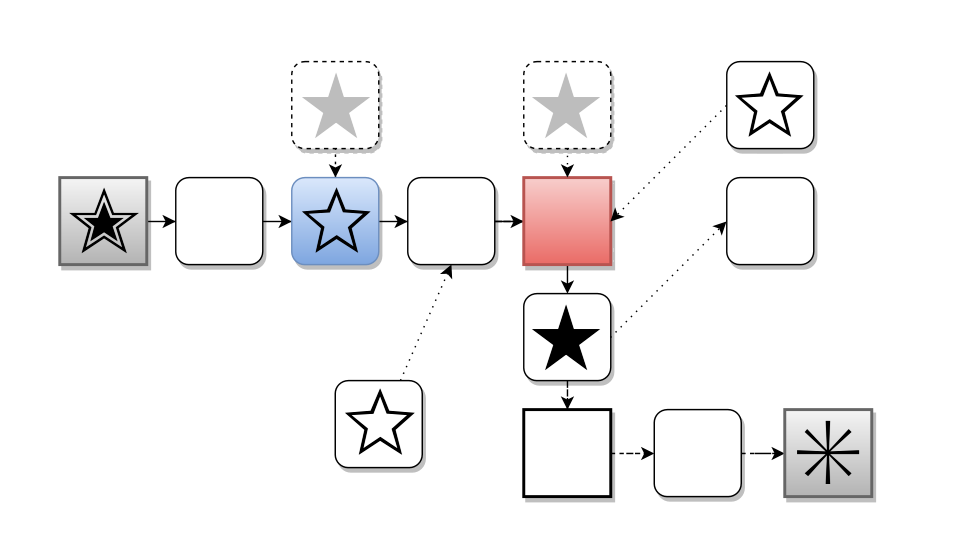
\includegraphics[scale=0.2]{./pictures/chain.png}
\end{figure}
\column{0.5\textwidth}
\begin{itemize}
\item определение цели для фигуры
\item построение траектории - подцепи-0
\item определение проходимости траектории
\item построение подцепей высших порядков
\end{itemize}
\end{columns}
Так как цепи весьма вариативны, необходимо выбрать оптимальное поддерево подцепей для цепи - произвести локальную оптимизацию.
\end{frame}

\begin{frame}{Формализация: оптимизация при построении}
\begin{columns}
\column{0.5\textwidth}
\begin{figure}
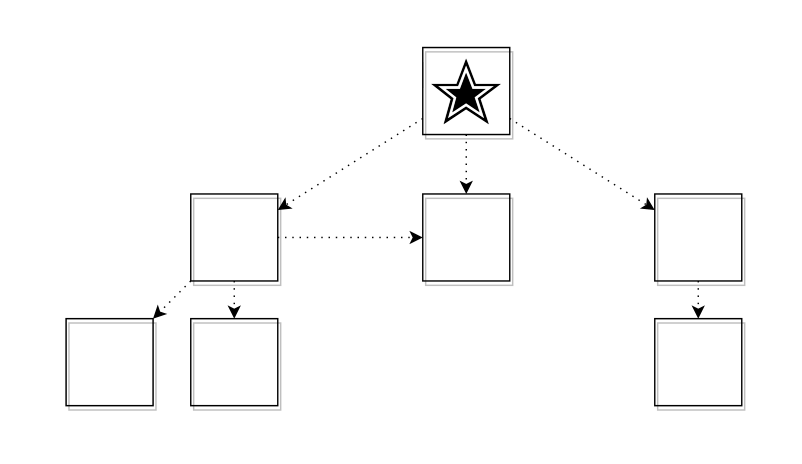
\includegraphics[scale=0.2]{./pictures/piece.png}
\end{figure}
\column{0.5\textwidth}
\begin{itemize}
\item квадраты - поля доски
\item с каждым полем связаны цепи
\item количество и качество цепей вляет на вес хода
\end{itemize}
\end{columns}
Глобальная оптимизация заключается в уточнении оценки для фигур по числу цепей, что может повлиять на уже построенные цепи
\end{frame}
